\maketitle
\tikz[remember picture,overlay] \node[opacity=0.5,inner sep=0pt] at (current page.center){\includegraphics[width=\paperwidth,height=\paperheight]{pic-title3}};
\clearpage
\newpage
\tableofcontents
\newpage

\section{Introduction}
This document was created after the NSAC trad climbing course of August 2024, with the goal to collect all the useful "tips and tricks" that were learned over the week.\\
It's not a manual on how to trad climb and there's no guarantee for correctness.\\
Think for yourself and make your own decisions.\\
You can fetch the latest version of this document on \href{https://github.com/leonclx/tradnotes_24}{github}. Feel free to \href{mailto:leon.cyliax@gmail.com}{email} me if anything seems incorrect.\\
I'd like to thank my course mates Adam, Dick, Jalmar, Quinten, Rutger, as well as the instructor Jeffrey Meesters and the mountain guide Nicolas Bartalucci for an amazing week in the alps :) \\
Many thanks to the NSAC ZP and Noël Diepens for organizing this course. 

\section{Placements}
Making good placements is the most important part of trad climbing. 
\begin{itemize}
\item All lobes of the cam must be within their working range, with good contact to rock
	\begin{itemize}
	\item On a C4 cam, if one lobe has no contact the whole cam comes out
	\item Totem cams are bodyweight rated for 2 lobes, 4 lobes is better
	\item Ideal engagement is at edge tip of cam facing directly down
	\item Overcammed (cam too big for crack) is safe, but risk of not getting cam back
	\item Undercammed (cam too small for crack) is dangerous
	\item Check for good contact area (solid rock, not just barely touching a rock tip)
	\end{itemize}
\item Make a placement before you anticipate a climbing move
	\begin{itemize}
	\item Similar to sports climbing, don't clip in the middle of the crux
	\item Clip before/after a climbing move, in a good position (physically and mentally)
	\item After a hard move, can place bomber next cam and then remove previous placement (runout)
	\item In some cracks, can move cam along as you go (somewhat risky)
	\end{itemize}
\item Place the stem of the cam in the direction you expect a fall/load
\item Tap the rock with the bottom of your palm to check if it's loose
\item Don't take a cam and try to jam it in somewhere. Look calmly for a crack and take the correct one
\item Cracks that open up towards the climber aren't good for placements because the cam looses engagement when it moves a tiny bit out of the wall
\item Cracks that open up towards the wall also aren't good because the cam can walk into the crack and loose engagement
\item Cams are asymmetric: One side has 2 wide apart lobes, the other 2 close together
	\begin{itemize} 
	\item Try both orientations, sometimes one works better
	\item Horizontal cracks are preferred with placing the wide apart lobes at the bottom (more stable)
	\end{itemize}
\item Don't make bad placements, it's a bad habit. Try a different size/crack, or climb up/down
\item Nuts need good surface area on the sides and a tuck to set them in. Extend with more than a quickdraw or they come out
\item Cam walking can be reduced with extended quickdraws. Especially bigger ones walk
\item You can practice cam placements on a bolted route or on boulder/scrambling terrain
\end{itemize}

\subsection{Removing placements}
\begin{itemize}
\item Stuck cam: Try getting the lobes to move. Use force but in the right way
\item Nuts: Place nut tool from below and give it a tap in the direction where it comes out
\item Tricam: push in a bit and then use a nut tool to fish it out
\end{itemize}

\subsection{Trad anchor}
\begin{itemize}
\item Placements are rated from 1-4, higher being better
\item A trad anchor needs at least 8 points (summing the points of all placements)
\item Assume factor 2 lead fall and a bad anchor $\rightarrow$ both climbers fall all the way down. Anchor is important
\item 2 really good cams is perfectly fine, no need to make 4..6..8 placements
\item Any material used in the anchor is unavailable for the next leader, but better to place a bit more and then discuss with partner
\item Sling anchors need to be counterloaded w/ bodyweight to prevent being pulled up/away from rock
\item Can place extra cam to hold upwards force for leader fall. Pre-tensioning usually not needed.
\item \href{https://www.alpinesavvy.com/blog/try-a-girth-hitch-at-the-master-point}{Girth hitch master point}: Quick and easy to remove, but needs "magic X" (twisting one of the lines)
\end{itemize}


\subsection{Types of protection devices}
\begin{itemize}
\item SLCDs (spring loaded camming device), anything with a spring that returns to an expanded form automatically. Cams/Friends, ballnuts, DMM Dragons, Camalot C4/Z4, Totems..
\item passive protection (nuts, wires)
\item semi-passive devices (tricams)
\end{itemize}



\section{On the rock}
\subsection{Approach/Descent}
\begin{itemize}
\item Make clear decisions and align but don't stand around for minutes doing nothing
\item Move as a team. Say "stop that's the wrong way" instead of "I found a better way but you do you"
\item Take off some load (ropes/water) if a teammate is slower than the rest
\item Conditions affect approach: Snowfields? Wet rock?
\item Often conflicting information, different options for approach/descent
\item Transition between scrambling and climbing can be fluid, free soloing is dangerous
\item Walking efficiently
	\begin{itemize}
	\item Look a few steps ahead, not just at your feet
	\item Aim at the tops of rocks, so you can roll over
	\item Try to keep momentum, don't get stuck against uphill rock
	\item Don't overdo it, rocks might be loose
	\end{itemize}
\item Better to put on helmet too early than to forget it later on. Similar with harness
\end{itemize}

\subsection{During the climb}
\subsubsection{General tips}
\begin{itemize}
\item Belaying more fluidly: hold follower rope under tension against knee, can feel when need to take in
\item Keeping anchor clean is really important, don't put unnecessary bieners, take out ATC when done etc
\item If there's spaghetti at belayer soon after starting, stop and turn around
\item Traverse trick
	\begin{itemize}
	\item In traverse: bolt .. tricky move ....................... next bolt
	\item Put a prussik thru last bolt, other end clipped into rope
	\item Allows second climber to safely climb tricky move, then untie/remove prussik
	\item Prussik needs to go beyond crux (5m usually enough)
	\item Can also do this for yourself if leader didn't do it
	\item Easier and faster to place piece after tricky move, not always possible on slab
	\end{itemize}
\item When calling 112, tell them where and that high mountain rescue is needed
\item For microtraxion, have to be sure nothing goes into/against the teeth (ice/rock/dirt/stone)
\item Belaying with microtraxion is ok, but has to always be tight esp. near relais. See \href{https://www.petzl.com/US/en/Sport/Belaying-the-second-with-a-MICRO-TRAXION--beware-of-any-fall?ProductName=MICRO-TRAXION}{Petzl tech tip}
\item Snapper can't be used for anchor main point, but for 2nd point it's fine. Ensure gate not against rock
\item When aiding, clip lifeline to piece instead of asking for block from belayer. With a block, the piece gets loaded with twice the force compared to lifeline (both climber and belayer hang on it instead of just climber).
\item Evaluate anchor before loading it. Don't hang in something and then check if it's good..
\item There's a way to make an HMS (munter hitch) autoblock by putting a screwgate into it, see \href{https://www.alpinesavvy.com/blog/the-auto-locking-munter-hitch}{here}
\item In limestone it's harder to place than in granite. 6kN small cams not great for anchor
\item There's no place for ego on the mountain. Important to have discussion moments when needed
\item It's nice to take a hardshell as a leader, especially if the weather is unpredictable
\item Right above relais, need more pieces. Towards end of pitch, can have more runout
\item Consider consequences of lead fall: Falls into bergschrund or on ice? Pulls belayer down snowfield or into wall? Fall onto ledge or into overhang? How much runout is ok?
\item If there's a pieton, no reason to skip it. Use short quickdraws if leadfall risk
\item For a hard pitch, consider leaving weight at follower (waterbottle/food/backpack)
\item In a chimney, clip your backpack below your legs
\end{itemize}

\subsubsection{Harness organization}
Having a clearly organized harness makes climbing safer and saves time.
Imagine struggling in a difficult position, far above your last piece, desperately searching for the right cam on your messy harness...
\begin{itemize}
\item Place equipment you need in front of your harness, where it's easy to reach
\item Left/right is less important, keep some balance. For most, right side is easier to reach
\item Put less needed/bigger equipment towards the back where it gets less in the way
\item Anticipate equipment needed for pitch: finger crack cam size, many slings for arrête, big offwidth..
\item Put things you don't need in your bagpack. Example 5m prussik, big cams if not needed etc
\item Try to keep things clean/organized from the start instead of "doing it later", it's less effort overall
\item Gates out is objectively better than gates in because carabieners take space if the spine is at the hip
\item Empty your harness for the approach/descent because cams/slings can get stuck (falling risk)
\item Bringing too much equipment makes the harness messy. 5 screwgates are usually plenty, no need for 20 quickdraws etc
\end{itemize}


\subsubsection{Helping a weak follower}
\begin{itemize}
\item Tell them to prussik up. Useful for lots of friction in overhang or for hanging precisely near stuck cam
\item "The frog" aka "leg workout": put prussik on climber side and squat up. Good at ledges
\item Double rope: block on one end, climber pulls on other (needs communication)
\item 3-1 usually not enough, can go to 5-1 directly. Sometimes microtrax and own body as counterweight is enough
\item Quick 5-1
	\begin{itemize}
	\item Attach microtrax to tight climber rope with screwgate, 60cm sling basket hitched to anchor
	\item Put backup knot on brake side (5m, figure 8, clip to anchor)
	\item Wriggle ATC biener to unload into microtrax
	\item Rest of 5-1: line fixed at anchor, going thru biener of prussik on victim rope. Other end biener, fed thru belay side. See \href{https://www.alpinesavvy.com/blog/6-1-compound-pulleys-in-the-real-world}{here}
	\end{itemize}
\end{itemize}


\subsubsection{Efficiency/Faster}
\begin{itemize}
\item Safety first, speed should come naturally, but never at cost of safety
\item Just fast is not the proper word..more about controlled, efficient, focussed, systematic
\item Gain time not by climbing faster but by everything else..looking 3min at placements, taking long to build anchors, taking 15min to rack up before climbing
\item For taking decisions, not stand around for minutes doing nothing, also not just doing anything. Decisive but discussed
\item ATC efficiency trick: always have 2 screwgates on atc, clip anchor side to harness. Clip to anchor after stand, close screwgate. Do this before pulling rope in
\item Just do stuff. Don't be dreaming. Split tasks (one puts on climbing shoes, other feeds through rope)
\end{itemize} 

\newpage
\subsection{Lifeline considerations}
When arriving at an anchor, how do you attach yourself to it?
\subsubsection{Requirements}
\begin{itemize}
\item Adaptable in length. Can be 20cm for hanging belay or 2-3m for nice big ledge. Usually 20cm-1m
\item Dynamic, in case belayer slips while trying to move around a bit (fall on static sling very dangerous)
\item Quick and easy to use, not make harness too messy/get stuck
\item For abseiling/rescue/solving rope spaghetti: not be in rope system
\item Safe: 8mm dyneema w/ knots is weak and easily burned by rope running over it
\end{itemize} 

\subsubsection{Options}
\begin{itemize}
\item Extendable dynamic lifeline, for example petzl connect, kong slide. Always on belay loop
\item Static lifeline with multiple fixed lengths (120cm aramid sling, grivel belay chain, etc)
\item Using the rope with a clove hitch
\end{itemize} 


\subsubsection{Dynamic Lifeline}
\begin{itemize}
\item Nice when you get to anchor. Clip bolt, pull on rope, you can hang
\item Adaptable, but not as flexible as rope. Good for aiding
\item Dynamic, safe against slip/fall at anchor
\item Heavy, takes up space on harness. Sometimes annoying to put away
\item Outside of rope system. Safe against burning through
\end{itemize}

\subsubsection{Static sling lifeline}
\begin{itemize}
\item Nice when you get to anchor, bit worse than dynamic lifeline but still easy
\item 2-3 fixed lengths, belay can get uncomfortable
\item Not safe against slip/fall at anchor, have to always hang. uncomfortable, dangerous
\item Less heavy than dynamic lifeline, but similar 
\item Outside of rope system. Needs wide/thick nylon sling or aramid one, burning through hazard
\end{itemize} 

\subsubsection{Rope w/ clove hitch}
\begin{itemize}
\item More effort at anchor than lifeline, but can get efficient at it (practice both hands, both gate directions)
\item Very adjustable, even long distances. Clove hitch can be hard to untie
\item Dynamic, safe against slip/fall at anchor
\item Takes up no space on belay loop, can't get stuck behind cams/legs
\item Inside rope system, can't untie. Very safe, rope is stronger than slings
\end{itemize}

\subsubsection{Conclusion}
Nico (mountain guide) prefers clove hitch using the rope.\\
For myself I think using dynamic or static sling lifelines is a bad habit and adds unnecessary complexity.\\
You can try out all options and draw your own conclusion. \\
For clove hitch, tying with both strands instead of 1 is stronger and prevents rope asymmetry. Use a large screwgate (gravity loaded), ballocks can't be used one-handed.




\section{Tour planning}
A good practice for tour planning is to get information from multiple sources. Don't trust one topo, but look it up on camptocamp. Check camptocamp outings, \textbf{ask the hut guardian}, check UK climbing forums. Topos at the hut can have additional handwritten information.
\subsection{Weather}
\begin{itemize}
\item Don't only look at the forecast, also look at how predictable the weather is
\item Meteoblue Arome (in multimodel) is best for predicting storms
\item Just rain is annoying but not that dangerous. Thunder is really dangerous
\item Use both meteoswiss/meteoschweiz and meteoblue
\item During the day, keep looking up. Are clouds moving towards? Dark/gray tall clouds (cumulonimbus) or high faint ones (cirrus)?
\item Better to check weather after breakfast instead of during/before. Can still change
\end{itemize}

\subsection{3x3}
Columns: Terrain, Conditions, Team. Rows: At home, At the start of the route, During the route.\\
See also \href{https://nkbv.nl/kenniscentrum/3-x-3-zomer-risicomanagement-in-alpien-terrein.html}{NKBV 3x3 zomer}

\subsection{Plan B}
It's useful to have a backup plan ready in case some unpredictable thing changes. Some examples:
\begin{itemize}
\item Weather prediction at 06:00 is better than last night vs worse/earlier rain
\item There's a slow team in front vs there's an empty route
\item Team member had a slight headache which remained vs team member feels a lot better
\end{itemize}

\subsection{Gear planning}
\begin{itemize}
\item Cams of size 4 and above are only needed if it says in topo
\item "1 rack" in topo usually assumes double middle sizes (gray, purple, green)
\item Better to bring too much cams and not need them than too little and be unsafe
\item Don't trust the topo too much regarding bolt location, gear quantity etc
\item Likewise, better to bring crampons/pickel and not need them than fall off snowfield
\item Leave C shoes/crampons below and abseil down? Or take with and walk down?
\end{itemize}

\subsection{Time estimation}
For time estimation it's good to leave margin because some things cannot be predicted precisely beforehand. For example rain could start at 12:00 or at 15:00, the 4c in the topo could feel like a 5c.\\
As the day goes on, those uncertainties usually become more clear.
\subsubsection{Approach/Descent}
\begin{itemize}
\item Times for approach and descent are usually listed in the topo
\item If the path is difficult to find, it's easy to loose 15min-30min (or more)
\item Naismiths hiking rule states 1h per 5km flat and 1h for 600m height (summed together)
\item Using only height meters and steep-ish terrain: 300-400m/h
\item Hiking with a heavy backpack is slower, especially when ascending
\item Some apps (eg Swisstopo) allow drawing lines to estimate hiking time
\item At the start/end of the route you can expect 5-10min to uncoil rope, put on shoes, organize harness
\item Well-prepared, aligned team: 30min for wakeup to out door. Inefficient: 1h, 1h30..
\item Taking a food break right before 100m height gain is miserable
\end{itemize}

\subsubsection{Climbing}
The general rule of thumb is 30min for climbing and 15min for abseiling each pitch.
\begin{itemize}
\item If the climbing is hard, more time is needed. Example 1st pitch 6a+ slab, wet shoes, 3 leadfalls: 1h
\item Easy pitches that have unclear direction can also take a bit longer (route finding). Rope drag!
\item Pitch length can vary; some are 45m, some are only 20-25m
\item Is it a straightforward sport style pitch or an alpine style arrête?
\item An efficient team with a clear line can climb a lot faster than 30min per pitch
\item If there's a slow group in front it can cost hours
\item Consider the climbing conditions: wet slab/crack, cold hands/feets, type of climbing
\item Abseiling can go 10min per pitch, but if the rope gets stuck once that can cost 15-30min
\item Can set an alarm on phone for the turnaround time
\end{itemize}






\section{Getting down}
\subsection{Walking down}
Walking down is usually preferred over abseiling. It's not always better, just typically faster and safer.
\begin{itemize}
\item Keep an eye out for cairns, but don't blindly follow them. Similar for other people.
\item If you lost the path, go back and try to find it again. Don't keep going into mistakes, turn around
\item Look a bit ahead to see where you should end up
\item In couloir, either go one for one (takes long) or stick together. Beware of loose rocks
\item Consider consequences of slip/fall: to next ledge (broken ankle) or off cliff (dead)
\item Judge terrain and act accordingly: crampons, pickaxe, short simulclimb/belay, 10m abseil..
\end{itemize}


\subsection{Abseiling}
Abseiling is dangerous and how most climbers die. It's usually done after climbing, when tired.
\begin{itemize}
\item Abseil anchor
	\begin{itemize}
	\item Check sunfaded, still supple/not stiff, check behind prussik for cuts/damage
	\item joining 2 pietons: single overhand fed thru for both, another one for abseil metal point (equalized). More good info \href{https://www.alpinesavvy.com/blog/retreat-anchors-alpine-climbing}{here}
	\item no metal/maillon rapide: one way ticket. OK for you, but rope burns prussik when pulling
	\item abseil on single snapper? possible, but check gate away from rock, be careful
	\item if you see bad/old sling, just cut it away
	\end{itemize}
\item Going back up on rope
	\begin{itemize}
	\item Only works in slow mode, with ATC teeth facing downwards
	\item Start by putting long prussik above ATC, for stepping in
	\item Step up, clip ATC guide mode ring to belay loop w/ screwgate
	\item Put backup knot below abseil prussik, remove abseil prussik
	\item Step up, pull rope through ATC, move foot prussik up. Repeat
	\end{itemize}
\item Joining knot (double rope), "european death knot"
	\begin{itemize}
	\item No crosses in knot, has to be dressed correctly
	\item Has to be very tight. pull on 4 strands individually
	\item Needs sufficient tail of 30-50cm. Don't make it longer, risk of setting up rappel on tail (deadly)
	\item Knot should be below maillon rapide, less risk of getting stuck
	\end{itemize}
\item Stopper knots
	\begin{itemize}
	\item Single overhand knot: Nico thinks not enough. Can come undone, rolls
	\item Barrel knot: Bit bigger, safe enough. Small enough not to get stuck
	\item Bigger knots: More risk of rope getting stuck from below
	\item Risky but possible: no stopper knots. Has to be clearly communicated. If next relais isn't visible/clear, put them in. Guides dont tie stopper knots usually, unless they dont see anchor
	\item Common mistake: pull rope thru, it falls down..oh nice it's already hanging. But: no stopper knot
	\end{itemize}
\item Rope control
	\begin{itemize}
	\item First abseiler doesn't remove prussik until 2nd is at relais
	\item Can extend prussik w/ 120cm sling if rope is slightly too short
	\item Risk in overhang or with wind: loosing control of rope
	\item Granite has high risk of getting rope stuck
	\item Rope stuck from below: don't pull it tight like a nut, flick it
	\item Keep ropes apart at relais, risk of getting twisted against eachother
	\item 1st abseiler can take rope with, coiled up on side of harness. Start on stopper knot end, coil up over head, use extended sling to clip to harness. Cams/Nuts tend to get stuck in rope carried like that. Can't get ends stuck like this.
	\item If 1st abseiler always has to solve rope spaghetti, it's not efficient
	\item Make shorter abseils if terrain is flat (reduce risk of rope stuck)
	\end{itemize}
\item Procedure
	\begin{itemize}
	\item Always partner check both stopper knots, the joining knot, which side to pull
	\item Abseil setup has to be clean: No twists, no prussik getting into ATC, no hair into ATC..
	\item 1st has to find next relais, keep control of rope ends, prepare next abseil
	\item When 1st arrives at next relais, should clip extra screwgate to share for lifelines
	\item 2nd has to not feed abseil rope through sharp V (rope stuck), clip lifeline on pull side
	\item Common mistake: 2nd arrives, clips lifeline. Immediately forgets which to pull. Use separate sling?
	\item At next relais, 1st can already prepare next abseil by putting pull side thru maillon, removing stopper knot on other rope
	\end{itemize}
\item Rope stuck above on one end, right after loosing other end? Tie one end to relais, prussik up stuck rope but place cams below. Rope suddenly gets unstuck, will fall in cams
\item Safety over efficiency, if you rush too much, it will cause mistakes and just end up costing more time
\end{itemize}

\subsection{Thunderstorm}
\begin{itemize}
\item In case there's a thunderstorm, just leave everything and get down
\item Leave cams behind, it's not worth your life. Leave the rope too
\item Stay away from via ferrata/metal. Throw metal stuff away, especially if you hear buzzing

\end{itemize}


\section{Glacier/C1}
\subsection{Crevasse rescue}
\begin{itemize}
\item make a T, with sling just as deep as other
\item ensure dead man orthogonal to where rope runs, but also orthogonal to snow slope
\item first priority is sitting/holding securely. Then build deadman nearby
\item microtrax at top to attach to dead man
\item how good is snow? try putting fingers/fist into. denser is better
\item at crevasse, put sth under rope to prevent cutting deeper
\item unconscious victim? call emergency, reach victim quickly
\item if possible, drop biener w/ 2 strings, not always easy
\item put own lifeline prusik on tight rope
\item 3 to 1 if alone probably not enough, probably 5 to 1 needed
\item 7 to 1 careful not strangulating victim
\item practice w/ snow covered crevasse much different from bare crevasse
\item keep rope tight while walking
\end{itemize}

\subsection{Misc}
\begin{itemize}
\item Going up steep snow field: Put weight on top of pickel, don't grab shaft but lean on top. Most weight on feet
\item Edge of glacier is most dangerous, this is where most of the movement is. Keep away
\item Don't pull on big rocks near glacier edge
\end{itemize}


\section{Reflection}
After the tour when you're back at the hut/camping it's good to sit together with everyone and reflect on the day.
\begin{itemize}
\item Keep chronological order: approach, start of climb, during climb, descent
\item Discuss things that went well, things that could go better
\item Was the time planning correct? Were there any dangerous/unsafe things?
\item During the tour is not the right time for starting heated discussions
\item Be honest about mistakes and don't look for blame, instead discuss how to prevent them for next time
\end{itemize}


\newpage
\tikz[remember picture,overlay] \node[opacity=0.95,inner sep=0pt] at (current page.center){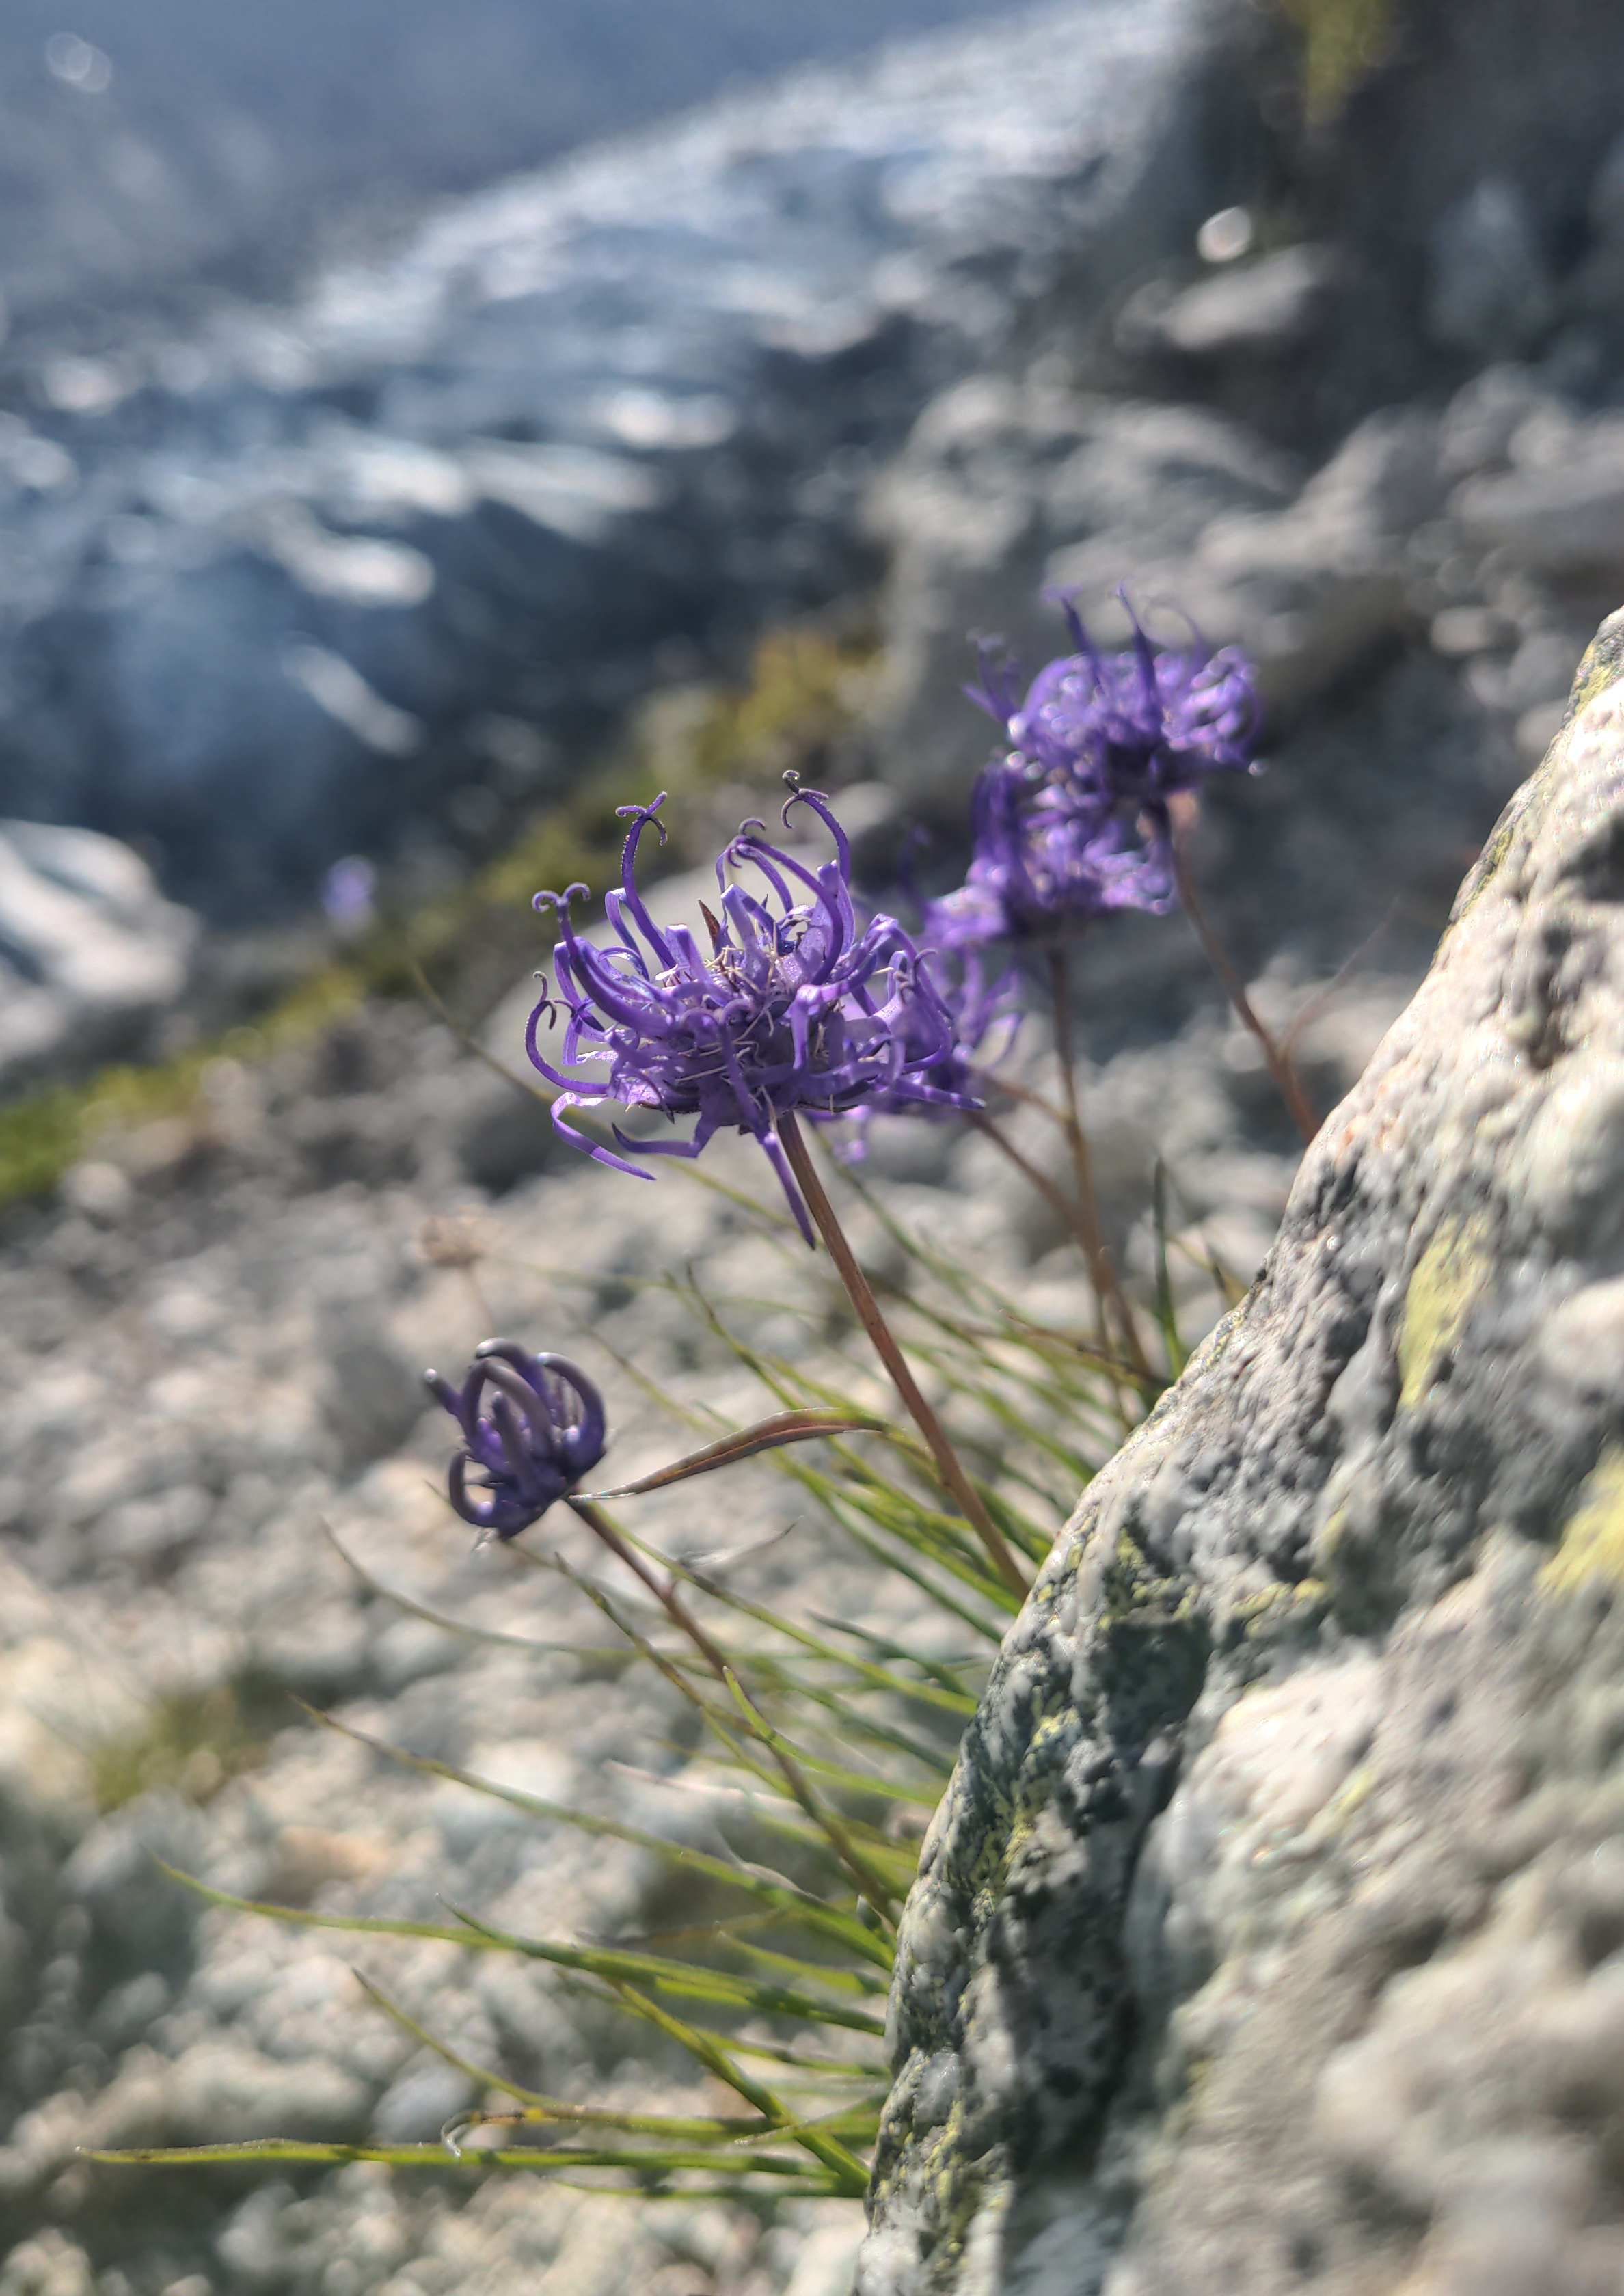
\includegraphics[width=\paperwidth,height=\paperheight]{flwr}};


